\chapter{Introduction} \label{chap:intro}

The study of galaxies, their formation, and evolution has been a cornerstone of astrophysics for over a century. One of the fundamental ways to describe galaxy properties and infer galaxy evolution is through its structure (morphology). This concept has a long history of development, starting with the earliest observations of galaxies and continuing up to the present as one of the primary methods we use to study galaxies. This thesis, titled "Investigating Galaxy Morphology in Large Surveys Using Novel Machine Learning Frameworks" pursues:-

\begin{itemize}
    \item Development of novel machine learning frameworks to study galaxy morphology
    \item Application of these new tools to large publicly available surveys
    \item Use of these unprecedented sample sizes to shed new light on the formation and evolution of galaxies. 
\end{itemize}

This chapter will start with a brief historical outline of how galaxy morphology has been used to study galaxy formation and evolution. We will discuss the different techniques used to study galaxy morphology and how they have evolved over time. Finally, we will discuss the critical drawbacks of existing techniques and gaps in the existing literature that we hope to address with this thesis. 

\section{A Brief History of Galaxy Morphology} \label{sec_intro:history}

\subsection{Early Observations} \label{sec_intro:early_obs}

The systematic study of galaxy morphology has its roots in the early $20^{th}$ century. Before this period, galaxies were often referred to as ``nebulae", a term used to describe any diffuse astronomical object, including galaxies, star clusters, and gas clouds. During this period, the study of galaxies remained largely descriptive, focusing on cataloging and general descriptions of structure. Prominent figures in this early period included Charles Messier, William and John Herschel, who identified and located galaxies by their resolved structure, as seen by eye. The true nature of these ``nebulae" as separate galaxies outside our own Milky Way was not widely accepted until the 1920s.

It is interesting to note that early descriptions of galaxy structures can be traced back to the pre-telescopic era. The Persian astronomer Abd al-Rahman al-Sufi, for instance, described the Andromeda nebula as a ``small cloud" in the $10^{th}$ century \citep{kepple_98}. 


\subsection{Key Breakthroughs Powered by Technological Advances} \label{sec_intro:technology}

Just like this thesis will aim to demonstrate, major technological advancements have always been a key component in characterizing galaxy morphology better. The late $19^{th}$ century and early $20^{th}$ century saw significant technological advances in many fields, including better telescopes and the advent of photography ---  allowing astronomers to examine the morphology and structure of external galaxies in more detail for the first time \citep[e.g.,][]{wolf_08,lundmark_26}. This ultimately led to Edwin Hubble's classification system for galaxies based on their visual appearance, now known as the Hubble sequence \citep{hubble_1926}. 

The basic Hubble sequence categorized galaxies into two main types: ellipticals and spirals.  Elliptical galaxies, characterized by their smooth, featureless light distribution and ellipsoidal shape, were further classified based on their ellipticity. Spiral galaxies, characterized by their flat, rotating disk component with spiral arms, were divided into normal spirals and barred spirals, depending on whether or not they exhibited a central bar structure. Hubble, and the astronomers who followed him, could classify most nearby bright galaxies using this system. As the $20^{th}$ century progressed, the development of morphological classification methods continued. Some revisions and refinements to the Hubble sequence were proposed, including the introduction of criteria like bars, rings, and other internal features that were prominent on photographic plates of galaxies \citep[e.g.,][]{devac_59}. Also, systems were developed to classify galaxies based on the form of their spiral arms and the clumpiness of light in these arms \citep[e.g.,][]{vbg_60,vbg_76,elmgreen_87}.

The next breakthrough in studying galaxy morphology came with the advent of photometric photometry and charged-coupled devices (CCDs) --- these further revolutionized the study of galaxy structure by allowing for detailed quantitative measurements of light distributions in galaxies. These enabled \citeauthor{de_vac_48} to realize that most massive elliptical galaxies follow the same fundamental light distribution --- now popularly referred to as the ``de Vaucouleurs profile" \citep{de_vac_48}. 

This early work by \citeauthor{de_vac_48} was later expanded on by many in the 70s and 80s. \citet{sersic_63} demonstrated that one could use a more general form of light distribution that could be used to describe both disks and massive ellipticals. \citet{kormendy_77} later used this general formalism to decompose light from a single galaxy into disk and bulge profiles. 

This large body of early breakthroughs provided the basis for modern galaxy morphology studies. They have enabled a decades-long endeavor in measuring the light profiles of galaxies in both the nearby and distant universe that continues even to this day. This, in turn, has powered a series of breakthroughs in understanding how galaxies form and evolve, which we discuss in the next section. 

\subsection{Early Impact on Understanding Galaxy Evolution} \label{sec_intro:gal_evo}
In the mid-1900s, as astronomers began cataloging the structure of more and more galaxies, they started to notice and investigate how the morphology of galaxies was correlated with other fundamental properties of galaxies. These observed correlations powered early efforts to understand how the observed features of galaxies can be explained by invoking physics. Studying such correlations has remained important even to this day, as we will show later in Chapters \ref{ch:gamornet} and \ref{chap:morph_den}.

One of the key insights derived from such early studies was the correlation between the morphology of a galaxy and its stellar population properties. Astronomers such as \citeauthor{holmberg_58} found that nearby elliptical galaxies are typically massive, consist mainly of old stars, and exhibit little to no ongoing star formation \citep{holmberg_58}. In contrast, nearby spiral galaxies contain significant populations of young stars and are actively forming new stars. This segregation of morphology in the local Universe  suggested that the morphological type of a galaxy is closely linked to its star formation history and provided an important clue for understanding the physics of galaxy formation.

This correlation between morphology and stellar population has been used to investigate various physical processes driving galaxy evolution. For instance, it has been suggested that the cessation of star formation in early-type galaxies could be due to a lack of available gas, possibly as a result of gas consumption by star formation, gas expulsion by stellar or active galactic nuclei (AGN) feedback, or gas stripping by environmental effects. On the other hand, the ongoing star formation in late-type galaxies suggests that these galaxies have been able to retain or accrete gas, possibly due to their lower masses, lower densities, or more isolated environments. We refer the interested reader to \citet{morph_review} for a recent review of these topics. We will also explore this topic in Chapter \ref{ch:gamornet}.

Another early insight observed was the relationship between a galaxy's morphology and its local environment. This empirical relationship was first noticed by \citet{dressler_84} -- he found that elliptical galaxies are more common in high-density regions of the universe, such as the centers of galaxy clusters, while spiral galaxies are more common in low-density regions, like the outskirts of clusters or in the field. This observation suggested a strong link between a galaxy's environment and its evolution, a concept that has remained a focus of research in the field of galaxy evolution. In fact, in Chapter \ref{chap:morph_den}, we will present a novel result showing the correlation between the size of galaxies and the large-scale structure of the universe. 

The morphology v/s local-density relation has also led to the development of several theories of galaxy evolution. For instance, it has been proposed that galaxies in high-density environments undergo interactions and mergers more frequently, disrupting spiral structures and forming elliptical galaxies. Alternatively, the hot, dense intracluster medium in these environments could strip gas from galaxies, quenching star formation and leading to the passive evolution of spirals into lenticulars and ellipticals.

\subsection{The Revolutionary Impact of Large Surveys \& Powerful Instruments} \label{sec_intro:large_surveys}

Following the early developments noted in the previous section, the advent of large galaxy surveys --- such as the Sloan Digital Sky Survey \citep[SDSS; ][]{sdss_tech_summary} and the Cosmic Assembly Near-infrared Deep Extragalactic Legacy Survey \citep[CANDELS; ][]{candels_1}) --- revolutionized the study of galaxy morphology. These have been powered by increasingly larger ground-based telescopes and powerful space-based observatories, such as the Hubble Space Telescope (HST) and JWST. In this thesis, we will use data from SDSS, CANDELS, as well as the Hyper Suprime Cam Subaru Strategic Program \citep[HSC-SSP; ][]{hsc_design}. 

The large volume of data from these surveys has enabled detailed analysis of galaxy morphology. They have powered a renaissance in the analysis of galaxy structure, allowing us to use galaxy structure as a tool for deciphering how galaxy assembly occurs over cosmic time. They have helped establish that galaxies undergo substantial evolution over time. This evolution is evident in the rapid development of the stellar mass density of galaxies at $z > 1$. Remarkably, by $z = 1$, approximately half of all stellar mass has been formed \citep[e.g.,][]{bundy_05,mortlock_11}. In addition, we observe a broad array of star-formation histories across individual galaxies, coupled with the integrated star-formation rate density in the Universe's history reaching its zenith at $z \sim 2.5$ and experiencing a decline at both higher and lower redshifts \citep[e.g.,][]{shapely_11, madau_dickinson_14}. Yet, it is not trivial to develop  a clear understanding of the forces driving the genesis and development of galaxies based on these observations. 

These large surveys have been used to expand on and refine the early results noted in \S \ref{sec_intro:gal_evo}. Galaxy morphology has been demonstrated to be connected to various additional fundamental properties of galaxies and their environment, including galaxy mass, stellar kinematics, merger history, cosmic environment, and the influence of supermassive black holes \citep[e.g.,][]{Tremaine2002TheCorrelation, pozzetti_10, wuyts_11, Huertas-Company2016MassCANDELS,powell_17, shimakawa_2021, Dimauro2022CoincidenceGrowth}. Distributions of morphological quantities alone have been used to place powerful constraints on possible galaxy formation scenarios. And when combined with other physical quantities, they have been shown to provide key insights into evolutionary processes at play or even reveal the role of new physical  mechanisms that impact evolution \citep[e.g.,][]{Kauffmann2004TheGalaxies,Weinmann2006PropertiesMass,Schawinski2007TheGalaxies,vanderWel2008TheMass,Schawinski2014TheGalaxies}.

Theoretical frameworks propose several possibilities to comprehend how galaxies form and evolve, and these are now also being explored through massive hydrodynamical simulations. The current consensus posits that the genesis of galaxies could occur through various processes. These encompass the embedding of gas in dark-matter halos, in-situ star formation within collapsed galaxies, major and minor galactic mergers, and gas accretion from the intergalactic medium. All these processes significantly impact the structure of a galaxy, and thus galaxy structure and morphology represent one of the most efficient tools to study galaxy formation and evolution. In Chapters \ref{ch:gamornet} and \ref{chap:morph_den}, we will delve into the impact of these processes in more detail. 

We are, now, in fact, able resolve galaxies back to $z \gtrsim 9$ using JWST \citep[e.g.,][]{labbe_23,finkelstein_23, kartaltepe_23}. It has solidified the understanding that galaxy structure is significantly different in the early Universe compared with what we see in our local universe. It also reveals a progression from galaxies at the highest redshifts -- small, peculiar, and undergoing high star-formation rates -- to the relatively quiescent galaxies we find in the nearby Universe. There have also been some surprises --- JWST has revealed an unexpected population of red galaxies that appear to have redshifts of $z \sim 7 − 9$ and are very small ($\sim 200 pc$) with high masses of $\log M/M_{\odot} > 10$.

In summary, the study of galaxy morphology has come a long way since the early days of the Hubble sequence. From the initial classification of galaxies into ellipticals, spirals, and irregulars, we have developed a nuanced understanding of galaxy morphology and its role in galaxy evolution. The advent of large galaxy surveys has opened up new avenues for research and provided key insights into the correlation of galaxy morphology with other fundamental properties of galaxies and how galaxy morphology evolves over time. Thus, studying galaxy morphology continues to be a vibrant field that significantly impacts our understanding of galaxy formation and evolution. 


\section{Methods to Determine Galaxy Morphology \& Structural Parameters} \label{sec_intro:determining_morph}

The measurement of galaxy morphology has evolved significantly over the years, with methods ranging from visual classification to sophisticated computational techniques. This evolution has been driven by the increasing volume and complexity of astronomical data and advancements in technology and computational power.

\subsection{Visual Classification \& Citizen Science Projects} \label{sec_intro:trad_morph}

The most traditional approach to classify galaxies has been using visual classification. Major visual classification systems in use today are evolved versions of the early classification systems described previously in \S \ref{sec_intro:technology}. We refer the interested reader to \citet{buta_13} for a review of visual galaxy classification. 

Visual morphological classifications have been conducted on nearly all deep HST imaging since its inception \citep[e.g.,][]{vdb_96, lee_13, kartaltepe_15} and have been applied on JWST imaging as well \citep[e.g.,][]{kartaltepe_23}. It should be noted that there are limitations on how visual classifications can be used at higher redshifts, as it has not been conclusively established how a galaxy's apparent morphology changes with redshift effects versus actual evolution \citep[e.g.,][]{morph_review}. Furthermore, distant galaxies resembling ``elliptical" or ``disky" structures don't necessarily share the same characteristics as their local counterparts. Key features like size, light profiles, color, and star-formation rates differ within the same galaxy morphological type over time. Thus, when used by itself, a galaxy's visual morphological type does not necessarily imply a particular local galaxy type, nor does it dictate a specific formation history or scale.

In response to the ever-increasing volume of data in astronomy, the 2010s saw the advent of citizen science projects like Galaxy Zoo \citep{gzoo_original} --- these projects used online platforms to collate votes from thousands of non-scientists to classify large numbers of galaxies. Although citizen science projects have been successful in processing many surveys over the last decade, these will fail to keep up with the upcoming data glut in astronomy with the advent of even larger surveys such as The Vera Rubin Observatory Legacy Survey of Space and Time \citep[LSST;][]{lsst}, the Nancy Grace Roman Space Telescope \citep[NGRST;][]{ngrst}, and Euclid \citep{euclid}. Moreover, reliable  classifications using citizen-science projects require a decent signal-to-noise ratio, take time to set up and execute, and require an extremely careful de-biasing of the vote shares obtained \citep[e.g.,][]{gzoo_original,gzoo_candels}. 

To summarize, while visual classification has the advantage of being intuitive and flexible, it is also subjective and time-consuming. The classification can vary between observers, and it is impractical for upcoming large data sets containing billions of galaxy samples. Despite these limitations, visual classification has played a crucial role in studying galaxy morphology and has provided the foundation for more advanced classification methods. It will continue to provide key insights when applied appropriately on small interesting sub-samples selected from upcoming large surveys. 

\subsection{Parametric Measurements of Galaxy Structure} \label{sec_intro:parametric_measures}

As referred to in \S \ref{sec_intro:technology}, \citeauthor{de_vac_48} and \citeauthor{sersic_63} were among the first to use integrated light profiles to describe galaxy structures. These involve measuring the average intensity of a galaxy at a specific radius and then determining how this intensity changes as a function of radius. With the advent of CCDs and increased computational power, these parametric measures were widely adopted in extragalactic astronomy. In particular, the surface brightness profile introduced by \citet{sersic_63} found wide usage. This is often referred to as the \sersic{} profile, and the surface brightness for a galaxy with the profile is given by

\begin{equation}
\label{eq_intro:sersic_fn}
\Sigma(r) = \Sigma_e \exp \left[ -\kappa \left( \left( \frac{r}{R_e}\right)^{1/n} - 1 \right) \right] ,
\end{equation}

\noindent where $\Sigma_e$ is the pixel surface brightness at the effective radius $r_e$, $n$ is the \sersic{} index, which controls the concentration of the light profile, and $\kappa$ is a parameter coupled to $n$ that ensures that half of the total flux is enclosed within $R_e$. Note that $R_e$ is often referred to as a galaxy's ``effective radius" or ``half-light radius". The de Vaucouleurs profile is typically represented by $n = 4$ in standard canonical benchmarks, while exponential disks are characterized by $n = 1$. 

A quantitative description of galaxy morphology is typically expressed in terms of structural parameters, which can be derived from Equation \ref{eq_intro:sersic_fn}. These include the brightness (integration of Eq. \ref{eq_intro:sersic_fn}), shape ($n$), and size ($R_e$) --- they serve as fundamental parameters for galaxies and play a significant role in their structural analysis. 

Although the above framework has been used extensively to study the structure of galaxies, moving beyond single-\sersic{} component determinations by using separate components to analyze galaxy sub-structure (e.g., disk, bulge, bar, etc.) can provide us additional insights into the formation mechanisms of these components: bulges, disks, and bars may be formed as a result of secular evolution \citep[e.g.,][]{kormendy_2004, genzel_2008, sellwood_2014} or due to the interaction of disk instabilities with smooth and clumpy cold streams \citep[e.g.,][]{dekel_09a,dekel_09b}. As noted earlier, combining multiple \sersic{} profiles to describe galaxy morphology was initially introduced in the context of decomposing the light in a galaxy into disk and bulge-components \citep{kormendy_1979}. A relevant parameter for the description of bulge-disk decomposition is $L_B/L_T$, which quantifies the fraction of the total light in the galaxy contained within the bulge. Because the bulge-disk decomposition framework provides a better way to describe most (local) galaxies as opposed to single \sersic{} profiles, we will be using it extensively later in this work to both simulate light profiles of galaxies as well as to determine the structural parameters of real galaxies.

The above-described procedure of fitting analytic two-dimensional light profiles to galaxy images found wide adoption in the early $21^{st}$ century \citep[e.g.,][]{graham_03, kormendy_09, simard_11,vdw_12}. The procedure provided a uniform framework to describe galaxy structure and effectively compare the morphology of different populations of galaxies. 

The task of fitting the above-mentioned light profiles to galaxy data is typically performed using a handful of light-profile fitting programs --- such as GIM2D \citep{gim2d}, GALFIT \citep{galfit}, GALAPAGOS \citep{galapagos}, Morfometryka \citep{morfometryka}, and ProFit \citep{profit}. These codes have slight differences, but the broad structure is the same. They depend on the user specifying a model and the initial values for the parameters of the chosen light profile model (such as those described in Eq. \ref{eq_intro:sersic_fn}). The codes thereafter iteratively adjust the  model's parameter values to minimize the residuals and improve the fit. This process often uses optimization algorithms like the Levenberg-Marquardt algorithm or a Markov Chain Monte Carlo (MCMC) method. As the optimization continues, the code refines the parameter estimates until it converges to the best-fitting values. The convergence criteria can vary depending on the code implementation and user-defined settings.

Some of the above-mentioned also predict crude estimates of uncertainties --- however, as we will demonstrate in Chapter \ref{chap:hsc_morph}, these estimates are typically severe underestimations of the true uncertainty. These codes also typically suffer from the fact that the quality of the fit depends heavily on the input parameters. When dealing with millions of galaxies, such hand-refinement of input parameters is an impossible task. In upcoming sections, we will delve deeper into some of these challenges and potential solutions. 

Despite these challenges, these codes represent simple methods for measuring the light profile of galaxies and have played a key role in the last two decades in helping us to understand the evolution of galaxy structure.

\subsection{Non-Parametric Measurements of Galaxy Structure} \label{sec_intro:non_parametric_measures}

Although not a focus of this thesis, for completeness, we provide a quick description of non-parametric methods to describe galaxy morphology. Non-parametric techniques broadly refer to a collection of statistical techniques that do not rely on specific predefined models or assumptions about the functional form of the galaxy's light profile. Instead, these methods aim to describe the structure of galaxies based on their observed properties.

These methods  originated in the photographic era, with early attempts by \citet{morgan_62} to quantify light concentration in galaxies. However, comprehensive quantitative measurements did not occur until the mid-1990s \citep{rix_95,conselice_97}. Currently, the most commonly used non-parametric methods for measuring galaxy structure include the concentration (C), asymmetry (A), clumpiness (S) system (CAS system), as well as similar parameters introduced by \citet{takamiya_99, papovich_03, abraham_03, lotz_04}. These parameters aim to capture the main characteristics of galaxy structures without assuming a specific underlying form, as is the case with model fitting described in \S \ref{sec_intro:parametric_measures}. Concentration measures the compactness of a galaxy's light distribution by quantifying the ratio of light within a specific radius to the total light. Asymmetry measures the deviation of a galaxy's appearance from perfect symmetry by comparing the pixel values of the galaxy with those of its mirror image.

Two other popular non-parametric measures happen to be the Gini Coefficient and M20 --- these have typically been used to find galaxies of broad morphological types, especially galaxies undergoing mergers \citep{abraham_03, lotz_04}. These parameters measure the relative distribution of light within pixels and do not involve subtraction, as is used for the asymmetry and clumpiness parameters, and therefore in principle, may be less sensitive to high levels of background noise. The Gini coefficient assesses the inequality in the distribution of pixel values within a galaxy image. It measures the cumulative distribution function of the sorted pixel values and indicates how uniformly or unevenly the light is distributed. M20 measures the concentration of the brightest $20\%$ of a galaxy's light --- it quantifies the contribution of the brightest regions to the overall luminosity and helps identify galaxies with prominent central concentrations.

Like parametric methods, non-parametric measures of galaxy morphology also suffer from many challenges:- a) Degeneracy and Interpretation: Non-parametric measures may not uniquely determine the underlying physical processes or structural components responsible for the observed morphology. Different galaxy structures can yield similar non-parametric measurements, leading to potential degeneracy and challenges in interpretation; b) Redshift Effects: Measuring galaxy structure at high redshifts introduces challenges due to limited resolution and sensitivity of observations. The interpretation of non-parametric measures becomes more complex as the morphological features may appear differently or be affected by observational biases; c) Subjectivity:  Non-parametric measures often involve subjective judgments or choices made during the analysis process. Decisions such as selecting regions of interest or setting thresholds can introduce variability and potential bias into the results.

\subsection{The Advent of Machine Learning} \label{sec_intro:ml_morph}

\begin{figure}[htbp]
    \centering
    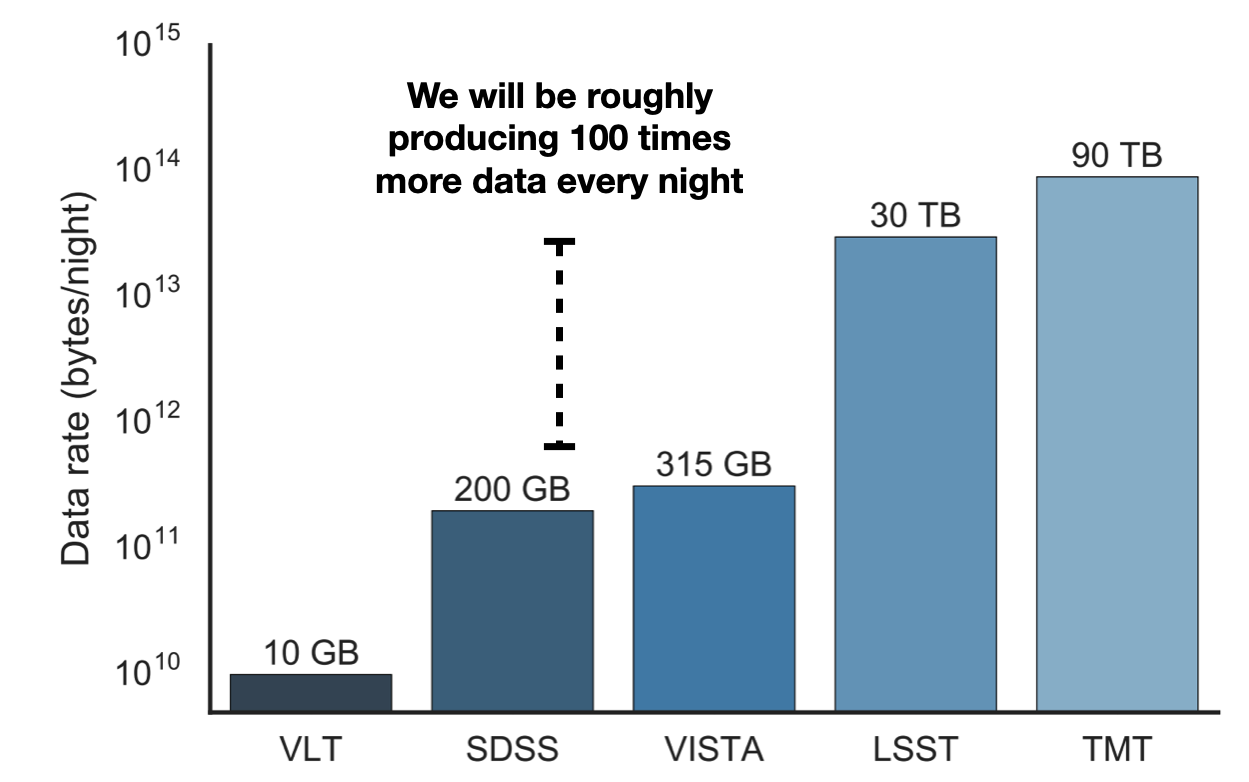
\includegraphics[width=0.6\textwidth]{data_volume.png}
    \caption{This figure has been adapted from \citet{kremer_17}. It shows the rate of data that will be produced (every night) by upcoming surveys such as the Rubin Observatory Legacy Survey of Space and Time (LSST) and the Thirty Meter Telescope (TMT) in comparison to existing surveys such as the Sloan Digital Sky Survey (SDSS). Note that the y-scale is logarithmic.}
    \label{fig_intro:data_volume}
\end{figure}


Over the next decade, we will witness a glut of new data in astronomy from a variety of new surveys such as Rubin-LSST, NGRST, and Euclid. Although we often talk about ``big data" in astronomy, actually quantifying the volume of data we will be generating is helpful. Figure \ref{fig_intro:data_volume}, adapted from \citet{kremer_17}, shows that these newer surveys will produce roughly 100 times more data every night than surveys in the last decade, such as SDSS. Therefore, to keep up with the data rate, existing algorithms must be scaled by a factor of 100. It is safe to say that none of the methods described previously in \S \ref{sec_intro:trad_morph} - \ref{sec_intro:non_parametric_measures} can be scaled to these levels. 

Note that it is not simply a matter of computational resources that prevent the above methods from being sped up. Arguably, even if the astronomy community could access 100 times more computational resources than it has in the past decade, it would still be nearly impossible to use these techniques to analyze these large data volumes. None of the above techniques were built to handle such large data volumes --- they require manual initiation, careful tuning, visual inspection of residuals, and post-processing for individual galaxies. 

Because of these challenges, over the last decade, machine learning (ML) has been increasingly used by astronomers to determine galaxy morphology. Early efforts in applying MLto galaxy morphology classification on a large scale were motivated by the data available from SDSS \citep[e.g.,][]{Ball2004GalaxyNetworks,Kelly2004MorphologicalSurvey,banerji_10}. These early methods involved the user selecting proxies, such as color, concentration index, and spectral features, as inputs to the ML models. However, since the relationship between these proxies and galaxy morphology was often unknown and potentially biased, these early networks were not optimal replacements for the traditional classification methods described previously. 

In the early years of the last decade, deep  convolutional neural networks\,(CNNs) revolutionized the field of image processing\,\citep[see][for an overview]{dl_1}. They are ideal for galaxy morphology classification as they eliminate the need to select morphological proxies manually. Instead, the network autonomously determines the most discriminative image features for distinguishing between different classes. The initial effort to employ CNNs for the morphological classification of galaxies emerged from the ``Galaxy Challenge" organized by Galaxy Zoo. Participating teams competed to replicate the vote distributions of each question in Galaxy Zoo 2 using a CNN. The top-performing entry was presented by \citealp{Dieleman2015Rotation-invariantPrediction}). This was followed by the work of \citet{Huertas-Company2015ALEARNING}, who used a CNN to reproduce visual classifications for CANDELS galaxies.

From these early attempts at using a CNN to classify galaxies morphologically (e.g.,  \citealp{Dieleman2015Rotation-invariantPrediction}) to the largest CNN produced morphology catalogs currently available \citep{Cheng2021GalaxyNetworks, Vega-Ferrero2021PushingSurvey}, most CNNs have provided broad, qualitative classifications, rather than numerical estimates of morphological parameters. Such studies typically entail classifying galaxies based on their morphological properties (e.g., based on whether the galaxy has a disk or a bulge or a bar, etc.) as opposed to predicting values of relevant morphological parameters that help characterize the galaxy (such as bulge-to-total light ratio, radius, etc.). By contrast, \citet{Tuccillo2018DeepFitting} used a CNN to estimate the parameters of a single-component \sersic{} fit, though  without uncertainties. Meanwhile, the computation of full Bayesian posteriors for different morphological parameters is crucial for drawing scientific inferences that account for uncertainty and thus are indispensable in the derivation of robust scaling relations  \citep[e.g.,][]{Bernardi2013TheProfile, vanderWel20143D-HST+CANDELS:3} or tests of theoretical models using morphology \citep[e.g.,][]{Schawinski2014TheGalaxies}. Thus, producing posterior estimates will significantly increase the scientific potential of morphological catalogs produced using CNNs. We will discuss this further in the next section. 

Using deep learning for determining galaxy morphology presents several challenges. One significant challenge is the availability and quality of labeled training data. Creating large and diverse datasets with accurate morphological annotations can be time-consuming and require expert knowledge. Another challenge is the interpretability of deep learning models. Understanding the decision-making process of complex neural networks and extracting meaningful insights from their learned representations can be difficult. Therefore, it is imperative to perform rigorous testing on such frameworks before mass adoption. Additionally, the prediction of uncertainties is a significant challenge for these models. In the next section, we will outline some of these challenges in more detail, followed by a description in the later chapters of how we address them.

\section{Outstanding Challenges \& Opportunities} \label{sec_intro:outstanding_challenges}
Despite the significant advancements in the study of galaxy morphology as outlined in \S \ref{sec_intro:history} \& \ref{sec_intro:determining_morph}, there remain several challenges and limitations with the current tools and methods.
These challenges are particularly pronounced in the context of large astronomical surveys. However, these challenges also provide the perfect opportunity for innovation; and, when applied to an appropriate dataset, can provide new insights into galaxy formation and evolution. In this section, we will outline the challenges we hope to address in this thesis. 

\subsection{Our ML Frameworks in the Context of Existing Tools} \label{sec_intro:ml_complementary}
As can be ascertained from the overview of the various methods provided in \S \ref{sec_intro:determining_morph} --- there is no ``best" method to determine galaxy morphology. Each method has its challenges and limitations. However, as the title of this thesis suggests, we are interested in determining morphology in large galaxy surveys --- that typically contain tens or hundreds of millions of galaxies. As we argued previously in \S \ref{sec_intro:ml_morph}, machine learning provides the best possible pathway to determine galaxy morphology for such big sample sizes. Therefore, for the remainder of this thesis, we will focus on developing novel machine-learning frameworks to determine galaxy morphology. 

\begin{figure}[htbp]
    \centering
    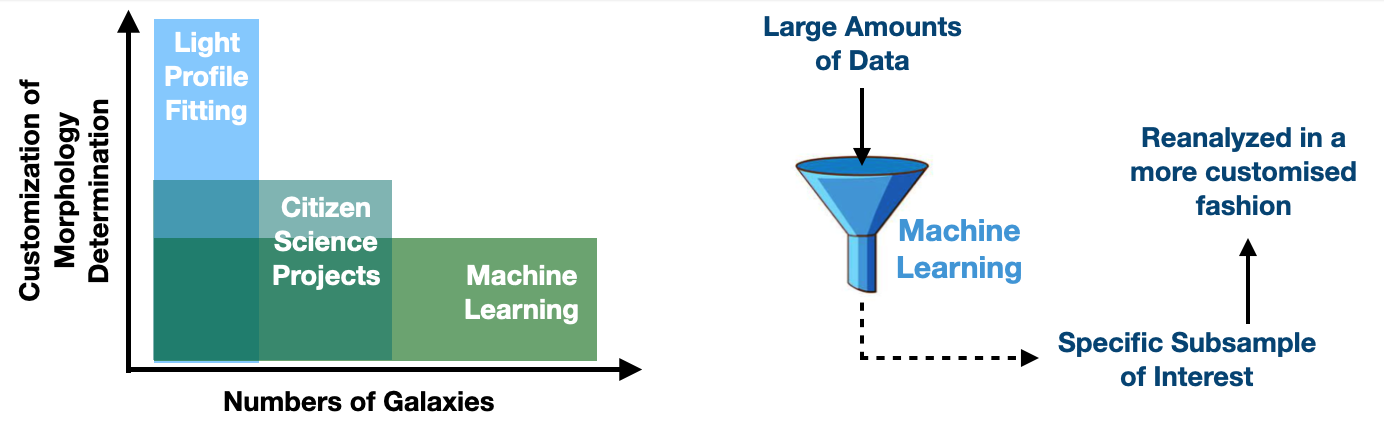
\includegraphics[width=\textwidth]{ml_workflow.png}
    \caption{The machine learning frameworks developed in this thesis are complementary to existing tools and methods. See text for more details.}
    \label{fig_intro:ml_workflow}
\end{figure}

At the very outset, let us discuss the placement of the novel tools we will develop in the context of existing tools to determine galaxy morphology. We have tried to demonstrate in Figure \ref{fig_intro:ml_workflow} two broad thought frameworks that can be used to appropriately choose when to use the new ML tools that we will develop in this thesis.

As the left panel of Figure \ref{fig_intro:ml_workflow} shows, one of the ways to determine the optimal method might be considering the total number of galaxies for which morphology determination is necessary and how flexible you want your algorithm to be among individual sample members (e.g., fitting each object with a different number/type of light profiles). In situations when one has a very limited number of galaxies ($\om(10^{2})$) and wants considerable flexibility in their morphology determination technique, light profile fitting might be the method of choice. Automated versions of light profile fitting (with the loss of model flexibility) might still be feasible for $\om(10^{3-4})$ galaxies. In a similar zone are citizen science projects which offer moderate flexibility and can be typically used on samples of sizes $\om(10^{5})$ to be completed within a reasonable timescale. However, for the billion galaxy samples of the upcoming decade, ML clearly should be the method of choice. 

Another way to use these novel ML frameworks is demonstrated in the right-hand panel of Figure \ref{fig_intro:ml_workflow}. ML frameworks can act like a funnel wherein large volumes of data can be processed quickly to obtain initial results. These can then be used to identify specific sub-samples of interest. Once this identification has been performed, astronomers may use their custom method of choice on the specific sub-samples for more detailed analysis. Therefore, the tools we will develop in this thesis are not meant to replace existing tools --- rather, they are new techniques that will work with existing tools to determine galaxy morphology in the next decade. 


\subsection{Key Challenges We Aim to Solve} \label{sec_intro:challenges}

Convolutional Neural Networks are adept at recognizing translation-invariant patterns in images in a hierarchical fashion and are thus often the natural ML method of choice for analyzing images. Therefore, we base all our new ML frameworks on CNNs. We will provide an in-depth introduction to all the components of our new CNNs in Chapters \ref{ch:gamornet} \& \ref{ch:gampen}. In particular, we refer the interested reader to \S \ref{sec:network_description} \& \S\ref{sec_c2:cnn_description} for more technical details about CNNs in general and our frameworks specifically. Additionally, please refer to \citet{mckay_03}, \citet{nielsen}, and \citet{chollet_21} for mathematical, concise, and Python-based introductions to neural networks, respectively.

As outlined in \S \ref{sec_intro:ml_morph}, deep CNNs were successfully applied for galaxy morphology determination for the first time around 2015 \citep{Dieleman2015Rotation-invariantPrediction, Huertas-Company2015ALEARNING}. Since then, they have become increasingly popular for determining galaxy morphology \citep[e.g.,][]{Tuccillo2018DeepFitting, Hausen2020MorpheusData, Walmsley2020GalaxyLearning, Cheng2021GalaxyNetworks, Vega-Ferrero2021PushingSurvey, Tarsitano2022ImageLearning}. However, despite having been around for half a decade, some significant challenges must be solved before these frameworks can be applied broadly to upcoming surveys. This section provides a broad outline of the challenges we hope to address with this thesis. 

\paragraph{Custom-Design \& Stress Testing} The move of astronomers from traditional methods to ML frameworks has largely been fuelled by technological innovations in computer science and machine learning. Given the current landscape of research in these fields in the recent past, the development of cutting-edge new tools has largely been driven by commercial applications/needs. Such commercial applications and needs often have different primary considerations than what has been traditionally important to astronomers (e.g., a network performing poorly on faint and smaller objects might be of bigger concern to astronomers; than to a researcher deploying similar frameworks for facial recognition). Besides, images used by astronomers may often have lower signal-to-noise ratios and specific peculiarities (e.g., the wide range of flux values pixels may have) compared to images widely used to train non-astronomy CNNs. Therefore, although it might be enticing to use these tools off-the-shelf as black boxes, this is extremely dangerous if we do not understand the accuracy, uncertainty, and biases of these algorithms \textit{specifically in the context of galaxy morphology determination}. Thus, in this work, we will focus on developing ML frameworks specifically for astronomical applications and extensively test and quantify errors, biases, and performance limits of these frameworks. These tests are essential to account for errors and biases properly while drawing scientific inferences from results produced by these frameworks. 

\paragraph{Need for Large Pre-Processed Training Sets} Almost all previous applications of using CNNs for galaxy morphology determination mentioned in the previous paragraph have one critical dependence --- they need large amounts ($\om(10^{5})$) of already-classified/analyzed images of galaxies to be trained. This presents two challenges:- 

\begin{itemize}
    \item training a CNN on visual classifications \textit{only} (either from domain-experts or citizen scientists) will result in the CNN having the same biases and inaccuracies that are inherent to visual classification that we discussed in \S \ref{sec_intro:trad_morph}
    \item If galaxy morphology catalogs for the next generation of surveys like Rubin-LSST, and NGRST will be built with CNNs, then we cannot expect large pre-classified datasets from the same survey to be available  for training. Although some works \citep[e.g.,][]{Cheng2021GalaxyNetworks} have proposed using images from the target survey and training labels from an older existing survey for training --- this presents the challenge that one is then limited to the depth, resolution, and noise limits of the older survey, whose labels are being used for training. 
\end{itemize}

In response to these challenges, in Chapters \ref{ch:gamornet} \& \ref{chap:hsc_morph}, we propose training CNNs first on simulations of the target data set followed by fine-tuning on a small amount of real data. We will demonstrate in those chapters that this approach presents dual benefits:- 
\begin{itemize}
    \item Simulations present the only situation where we can access the robust ``ground-truth" morphology. Therefore, they present the ideal dataset to both train CNNs and also evaluate their performance in comparison to other frameworks (e.g., we will demonstrate in \S \ref{ap:sec_c3:gapemn_v_galfit} that one of our ML frameworks outperforms traditional light profile fitting algorithms, especially for fainter and smaller galaxies).
    \item Training on simulations greatly reduces the amount of real data needed for training. We will demonstrate in Chapters \ref{ch:gamornet} \& \ref{chap:hsc_morph} how we can successfully train ML frameworks by using even less than $1\%$ of the total dataset for training. This provides a viable framework for using CNNs on large upcoming surveys like Rubin-LSST, NGRST, and Euclid.
\end{itemize}


\paragraph{Sensitivity of Models to Specific Data Sets} Early applications of CNNs to galaxy morphology classification typically involved training frameworks  targeted for a specific survey and then testing the CNN on the same survey \citep[e.g.,]{Dieleman2015Rotation-invariantPrediction, Huertas-Company2015ALEARNING, Tuccillo2018DeepFitting}. There was no attempt to check whether the same CNN framework can be applied to data from different surveys with varying resolution, PSF, and signal-to-noise ratio. This is a challenge if we have to design a new ML framework every time we deal with data from a different survey --- as this involves significant time, computation, and effort; and is not viable for the long term. In Chapter \ref{ch:gamornet}, we will present one of the first works, where we successfully apply the same CNN framework to both ground and space-based imaging and obtain state-of-the-art accuracy on both these data sets. 

\paragraph{Moving Beyond Classification to Parameter Estimation} From early attempts at using a CNN to classify galaxies morphologically (e.g.,  \citealp{Dieleman2015Rotation-invariantPrediction}) to the largest CNN produced morphology catalogs currently available \citep{Cheng2021GalaxyNetworks, Vega-Ferrero2021PushingSurvey}, most CNNs have provided broad, qualitative classifications, rather than 
numerical estimates of morphological parameters. Such studies typically entail classifying galaxies based on their morphological properties (e.g., based on whether the galaxy has a disk, a bulge, or a bar, etc). Although such classifications are useful, typically, distributions of structural parameters of galaxies have been essential to place powerful constraints on possible galaxy formation scenarios \citep[e.g.,][]{Kauffmann2004TheGalaxies,Weinmann2006PropertiesMass,Schawinski2007TheGalaxies,vanderWel2008TheMass,Schawinski2014TheGalaxies}. Therefore, it is essential to develop CNNs that can predict numerical estimates of structural parameters of galaxies. In Chapter \ref{ch:gampen}, we will introduce one of the first ML frameworks to do that. 

\begin{figure}[htbp]
    \centering
    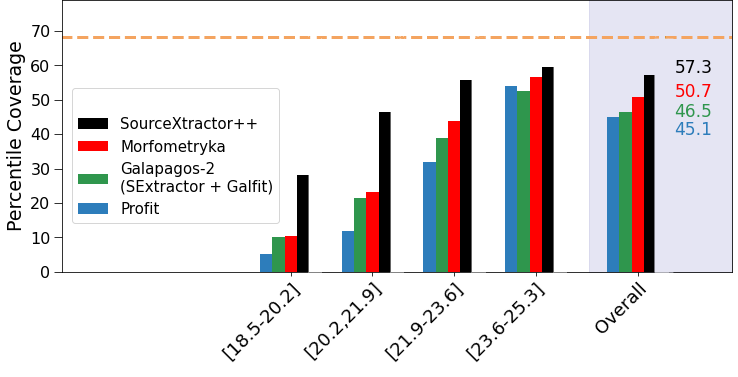
\includegraphics[width=0.9\textwidth]{cov_prob_euclid_wo_gampen.png}
    \caption{Traditional light profile fitting tools severely underestimate uncertainties --- by $\sim15-25\%$ overall and by as much as $\sim60\%$ for the brightest galaxies. This figure shows percentile coverage probabilities obtained by various light-profile fitting algorithms on simulated Euclid data \citep[][]{euclid_morph}. Percentile coverage probabilities in this figure refer to the fraction of times the true value predicted by each algorithm was within the central $1\sigma$ confidence interval --- ideally, the bars should align with the horizontal dotted line at $68.27\%$. The rightmost set of bars shows the values calculated on the entire dataset, while the other sets display values calculated on sub-samples of galaxies with specific magnitude ranges (AB mag, shown on the x-axis). We will demonstrate later in \S \ref{sec_c3:uncer_comp} that the uncertainties predicted by our ML frameworks provide a major breakthrough by remaining well-calibrated (with $<5\%$ deviation) for the entire range of magnitudes.}
    \label{fig_intro:uncertainties}
\end{figure}

\paragraph{Prediction of Robust Uncertainties} Along with parameter estimation comes the challenge of estimating robust uncertainties. The computation of full Bayesian posteriors for different morphological parameters is crucial for drawing scientific inferences that account for uncertainty and thus are indispensable in the derivation of robust scaling relations  \citep[e.g.,][]{Bernardi2013TheProfile, vanderWel20143D-HST+CANDELS:3} or tests of theoretical models using morphology \citep[e.g.,][]{Schawinski2014TheGalaxies}. Thus, producing posterior estimates is essential to significantly increase the scientific potential of morphological catalogs produced using CNNs. We note here that the prediction of uncertainties has been a persistent challenge in galaxy morphology irrespective of whether one is using traditional light-profile fitting tools outlined in \S \ref{sec_intro:parametric_measures} or ML tools outlined in \S \ref{sec_intro:ml_morph}. For ML tools, there have been no attempts at comprehensively constraining their uncertainties in the context of galaxy morphology, and traditional light profile fitting tools severely under-predict the amount of uncertainties as comprehensively demonstrated in Figure \ref{fig_intro:uncertainties}. Therefore, we make predicting robust uncertainties a key priority and introduce the first ML framework (in Chapter \ref{ch:gampen}) that can predict well-calibrated Bayesian posteriors for different structural parameters of galaxies. 

\paragraph{Multiple-Component Analysis} When not trained on visually classified images, most previous works using CNNs focused on recovered morphologies obtained from single-component \sersic{} fits of galaxies \citep[e.g.,][]{Tuccillo2018DeepFitting}. However, moving beyond single-component determinations by using separate components to analyze galaxy sub-structure (e.g., disk, bulge, etc.) can provide us additional insights into the formation mechanisms of these components \citep[e.g.,][]{kormendy_1979,kormendy_2004, genzel_2008, sellwood_2014}. In Chapters \ref{ch:gamornet}-\ref{ch:gampen} we will demonstrate how we can successfully recover morphological classifications and structural parameters for galaxies with disk + bulge components. To the best of our knowledge, this represents the first time it has been demonstrated that CNNs can be used to determine the morphology of multi-component galaxies.

\paragraph{Reducing the Impact of Bright Secondary Objects} Although the introduction of CNNs has accelerated morphology determination recently, some challenges related to data pre-processing have remained. One of these challenges has to do with making cutouts of proper sizes. Most trained CNNs require input images of a fixed size---thus, most previous work (e.g., \citealp{Cheng2021GalaxyNetworks, Vega-Ferrero2021PushingSurvey}) has resorted to selecting a large cutout size for which ``most galaxies" would remain in the frame. However, this means that for many galaxies in the dataset, especially smaller ones, typical cutouts contain other galaxies in the frame, often leading to less accurate results. A few examples are shown in Figure \ref{fig_intro:crowded_cutouts}. This problem is aggravated when designing a CNN applicable to an extensive range in redshift, corresponding to a large range of galaxy sizes. Lastly, most previous work has used computations of $R_e$ from previous catalogs to estimate the correct cutout size to choose. This is, of course, not possible when trying to use a CNN on a new, unlabeled dataset. To address these challenges, in Chapter \ref{ch:gampen}, we introduce a novel ML framework that can automatically crop cutouts to an optimal size before determining their morphological parameters. 

\begin{figure}[htbp]
    \centering
    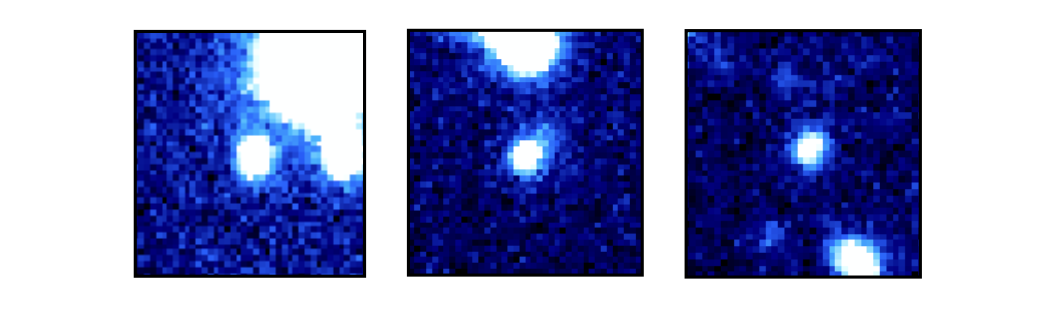
\includegraphics[width=0.9\textwidth]{crowded_cutouts.png}
    \caption{CNNs require cutouts of a fixed size; therefore, most previous uses of CNNs involved using a large cutout size that would encompass ``most galaxies". However, this leads to secondary objects being present in the frame, which can be a major source of spurious predictions. We introduce a novel ML framework in Chapter \ref{ch:gampen} that can automatically crop galaxies before determining their structural parameters.}
    \label{fig_intro:crowded_cutouts}
\end{figure}


\paragraph{Determining the Morphology of AGN Host Galaxies} None of the CNNs that have been used previously used to determine morphological parameters can be used on sources with Active Galactic Nuclei (AGN) --- this is because determining the morphology of AGN host galaxies requires careful decomposition of the light coming from the AGN to be separated from that of the host galaxy. Although not a focus of this thesis, we would like to point out that we have tested both frameworks we will introduce in Chapters \ref{ch:gamornet} \& \ref{ch:gampen} on AGN host galaxies. We have demonstrated that by combining the frameworks presented in this thesis with another generative machine learning framework, we can successfully determine the morphology of AGN host galaxies. We refer the interested reader to \citet{tian_23} for an extended description.

\subsection{New Insights into Galaxy Evolution} \label{sec_intro:gal_evo_opportunities}

In \S \ref{sec_intro:challenges}, we outlined some of the key technical challenges we will aim to solve. Our hope is that these key technical breakthroughs will provide the framework needed to analyze the morphology of the billion galaxy samples expected from future large surveys. The ultimate goal is to use these predicted morphologies thereafter as a tool to decipher galaxy evolution. 

As we will outline in later chapters, we have already applied our frameworks to a combination of ground and space-based galaxy surveys: SDSS, CANDELS, and Hyper Suprime-Cam Subaru Strategic Program (HSC-SSP). There are a plethora of ways in which the public morphological catalogs produced from this thesis can be used to investigate galaxy evolution. Here, we focus on two specific applications that we choose as the first applications of our produced catalogs. 

\paragraph{Deciphering the Role of Environment in Structural Evolution} As noted in \S \ref{sec_intro:gal_evo}, it was first observed in the late 1900s that galaxy morphology strongly correlates with the local environment. There is now considerable evidence showing that whether a galaxy is either elliptical or spiral depends to a large degree (in
the local universe) on the local density of that particular galaxy’s environment. The higher the density of the local environment, the more likely a galaxy is early-type and non-star-forming \citep[e.g.,][]{dressler_84, gomez_03, blanton_09}. Although the evidence gets more sparse at higher redshifts, the effect has also been shown to exist in the high redshift universe till $z\sim2-3$.

However, something that is not well-established at all is the variation of galaxy size with environment, especially at redshifts $z > 0.2$. Beyond the local universe, different studies have reported conflicting results, as summarized later in Table \ref{tab_c4:lit_survey}. While some studies have reported a positive correlation of radius with the environment for certain sub-populations of galaxies \citep[e.g.,][]{Cooper12,Lani13,Bassett13,Afonso19,Siudek22}; some studies have reported no correlation \citep[e.g.,][]{Huertas-Company13,Kelkar15,Gu21}; and some have reported negative correlation \citep[e.g.,][]{Matharu19,Chan18}. These conflicting results can largely be attributed to a host of different challenges that previous studies have faced:- a) lack of statistically significant sample sizes; b) the presence of systematics between measurements made from different samples (used in the same study);  c) not accounting for uncertainties in the measurements of galaxy radius. 

Our newly developed ML frameworks and the excellent imaging quality of HSC puts us in a unique position --- for the first time, we simultaneously have access to the radius measurements of millions of galaxies beyond the local universe, as well as measurements of environmental density covering $\sim360$ deg$^2$. This presents the perfect opportunity for us to present in Chapter \ref{chap:morph_den} the first comprehensive study of the variation of galaxy radius with large-scale structure beyond the local universe. 

The robustness of our new ML frameworks and the depth of the HSC data allow us to go up to $z\sim0.75$ and down to a mass completeness limit of $\log M/M_{\odot} \sim 8.5$ at $z=0.3$ and $\log M/M_{\odot} \sim 10$ at $z=0.7$. Using the full Bayesian posteriors predicted by our frameworks, we are able to incorporate the uncertainties in radius measurements into our correlation analysis. This allows us to confirm/reject the presence of correlations with very high statistical significance --- in most cases with $>5\sigma$ confidence. We posit in Chapter \ref{chap:morph_den}, how these observed correlations might be a result of both halo assembly bias as well as the greater rate of gravitational effects (such as mergers, and ram pressure stripping) in denser regions of the universe. 

\begin{wrapfigure}{R}{0.4\textwidth}
\centering
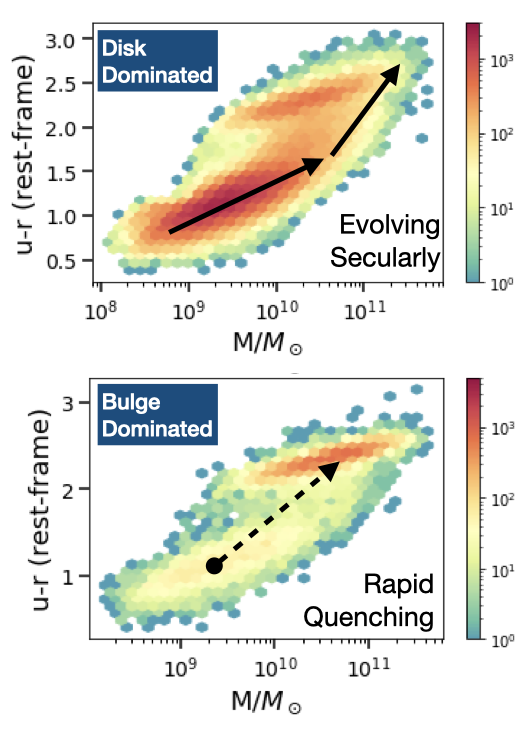
\includegraphics[width=0.4\textwidth]{sdss_cmd.png}
\vspace{-0.3in}
\caption{An example color-mass diagrams for SDSS $z\sim0$ galaxies from Chapter \ref{ch:gamornet}. Disk-dominated galaxies (top panel) are mostly blue until they reach high masses (and presumably high halo masses), at which point they evolve to the red sequence. In contrast, bulge-dominated galaxies (bottom panel) are predominately red, and appear to evolve rapidly from a short-lived population of rare, blue ellipticals that likely formed from major mergers of disky star-forming galaxies.}
\label{fig_intro:sdss_cmd}
\vspace{-0.2in}
\end{wrapfigure}

\paragraph{Revisiting the Connection between Galaxy Structure \& Star Formation} We know from large-scale surveys that both local and high-redshift galaxies show a bimodal distribution in the galaxy color-mass space\,\citep{strateva_01,baldry_04,baldry_06,brammer_09} with a ``blue cloud,'' a ``red sequence'' and a ``green valley.'' Galaxy color-mass diagrams are useful for studying galactic evolution, as the stellar mass of a galaxy indicates its growth over time, and the color tracks its rate of star formation. The standard interpretation of the bimodal color-mass distribution is that, because there are few galaxies in the green valley, star formation in blue cloud galaxies must be quenched rapidly, perhaps aided by emission from an AGN \citep{bell_04,faber_07}). Direct evidence of this AGN feedback remains murky, however \citep{harrison_17}.

Galaxy morphology adds a third interesting dimension to the color-mass space as shown in Figure \ref{fig_intro:sdss_cmd}. Because elliptical galaxies typically form in major mergers, and galactic disks usually do not survive them, 
morphology can be used as a tracer of the recent merger history of a galaxy. The observed bimodality in the color-mass diagram (as well as interpretations therefrom) comes from superposing distinct populations with different morphological types, as first shown by \citet{Schawinski2014TheGalaxies}, who used Galaxy Zoo morphological classifications to study local ($z\sim0$) galaxies. They suggested that there are two separate evolutionary tracks for galaxies: (1) major mergers forming ellipticals from disk-dominated galaxies, accompanied by AGN triggering and rapid quenching of star formation, and (2) slow, secular growth of disk-dominated galaxies until they reach a critical halo mass, after which the remaining cold gas is slowly consumed and the stellar population gradually reddens. At $z\sim0$, the latter population is an order of magnitude larger than the merger-created ellipticals. 

As we outline in Chapter \ref{ch:gamornet}, we aim to perform the morphology-color-mass analysis for a sample of SDSS $z\sim0$ and CANDELS $z\sim1$ galaxies. Our ML frameworks enable us to use a sample-size $2\times$ and $10\times$ larger than what had been done previously at $z\sim0$ and $z\sim1$, respectively. Larger samples are particularly important for bins with low statistics in order to establish the existence of galaxy formation pathways across the color-mass diagram (e.g., \cite{powell_17} were able to identify only 5 bulge-dominated galaxies in the green valley). We will use our ML-enabled large samples to:- a) confirm/refine the existence of galaxy evolution pathways on the color-mass diagram; b) put better constraints on the fractions of rare objects (such as massive red disks) and how these fractions evolve over cosmic time. 


\section{Outline of This Thesis} \label{sec_intro:thesis_outline}

Summarizing the information presented in \S \ref{sec_intro:challenges} \& \ref{sec_intro:gal_evo_opportunities}, below we present the key technical and science goals of this thesis:-

\begin{tcolorbox}[breakable,colback=blue!5!white,colframe=blue!75!black,title=\textbf{Key Technical Goals}]
\begin{itemize}
 \setlength\itemsep{-0.1em}
\item \textbf{Developing a technique to train ML frameworks without requiring large pre-classified training sets of real data}
\item \textbf{Developing ML frameworks which can be applied universally to data of varying resolution, signal-to-noise ratio, point spread function, etc.}
\item \textbf{Enabling ML frameworks to move beyond classification tasks and predict galaxy structural parameters along with robust Bayesian posteriors (i.e., values + uncertainties)}
\item \textbf{Moving beyond single component analysis to perform multi-component determination with ML frameworks}
\item \textbf{Reducing the sensitivity of ML frameworks of bright secondary sources by enabling them to automatically crop cutouts}
\end{itemize}
\end{tcolorbox}

\begin{tcolorbox}[breakable,colback=blue!5!white,colframe=blue!75!black,title=\textbf{Key Science Goals}]
\begin{itemize}
 \setlength\itemsep{-0.1em}
\item \textbf{Develop a publicly available catalog of structural parameters (along with uncertainties) for $\sim8$ million HSC Wide galaxies till $z=0.7$ down to $m < 23$}
\end{itemize}
\tcblower
\begin{itemize}
\setlength\itemsep{-0.1em}
\item \textbf{Perform the first comprehensive study of the correlation of galaxy radius with large-scale structure beyond the local universe}
\item \textbf{Use the above correlations to investigate the role of dark matter halos and galaxy mergers/interactions in the structural evolution of galaxies}
\end{itemize}
\vspace{-0.25in}
\DrawLine
\vspace{-0.15in}
\begin{itemize}
\setlength\itemsep{-0.1em}
\item \textbf{Use an order of magnitude larger sample than what has been used previously to revisit the connection between structure and star-formation at $z\sim0$ and $z\sim1$ using SDSS and CANDELS data respectively.}
\item \textbf{Use the above statistics to put better fractional constraints on the existence of rare morphological objects such as massive red disks}
\end{itemize}
\end{tcolorbox}

In Chapter \ref{ch:gamornet}, we will introduce a new ML framework called Galaxy Morphology Network (\gamornet) that can be used to predict morphological classes of multi-component galaxies. We will demonstrate how \gamornet{} can be successfully applied to both space and ground-based imaging data from SDSS and CANDELS without needing a large training set of real galaxies. We will finally use the predicted SDSS and CANDELS morphological classifications to revisit the connection between galaxy morphology and star formation.

In Chapter \ref{ch:gampen}, we will introduce a novel ML framework called Galaxy Morphology Posterior Estimation Network (\gampen{}) that can:- a) predict full Bayesian posteriors (i.e., values + uncertainties) for different structural parameters of galaxies (including parameters from disk + bulge decomposition); b) automatically crop galaxies to an optimal size before performing morphology determination. We will extensively test this novel framework on simulation HSC imaging.

In Chapter \ref{chap:hsc_morph}, we will apply \gampen{} to HSC galaxies to produce a publicly-available morphological catalog for $\sim 8$ million galaxies in the Hyper Suprime-Cam (HSC) Wide survey with $z \leq 0.75$ and $m \leq 23$. We will put \gampen{} head-to-head against existing light profile fitting frameworks (like GALFIT) to compare their performance, as well as demonstrate the highly accurate nature of \gampen{}'s posteriors.

In Chapter \ref{chap:morph_den}, we will use the structural parameters of a sub-sample of $\sim3$ million galaxies from Chapter \ref{chap:hsc_morph}. We will correlate these parameters with large-scale structure density measurements over $\sim360$ deg$^2$. This represents the first comprehensive study of the variation of galaxy radius with large-scale structure beyond the local universe

Finally, in Chapter \ref{chap:conc}, we will present our conclusions and the path forward. 